\chapter{Analisi dei requisiti}
\label{chap:AnalisiRequisiti}
\section{Requisiti funzionali}
In questa sezione riassumo tutti i requisiti funzionali emersi.
All'interno della tabella seguente saranno anche presenti le priorità assegnate a ciascun Item.
\begin{figure}[h]
    \centering
    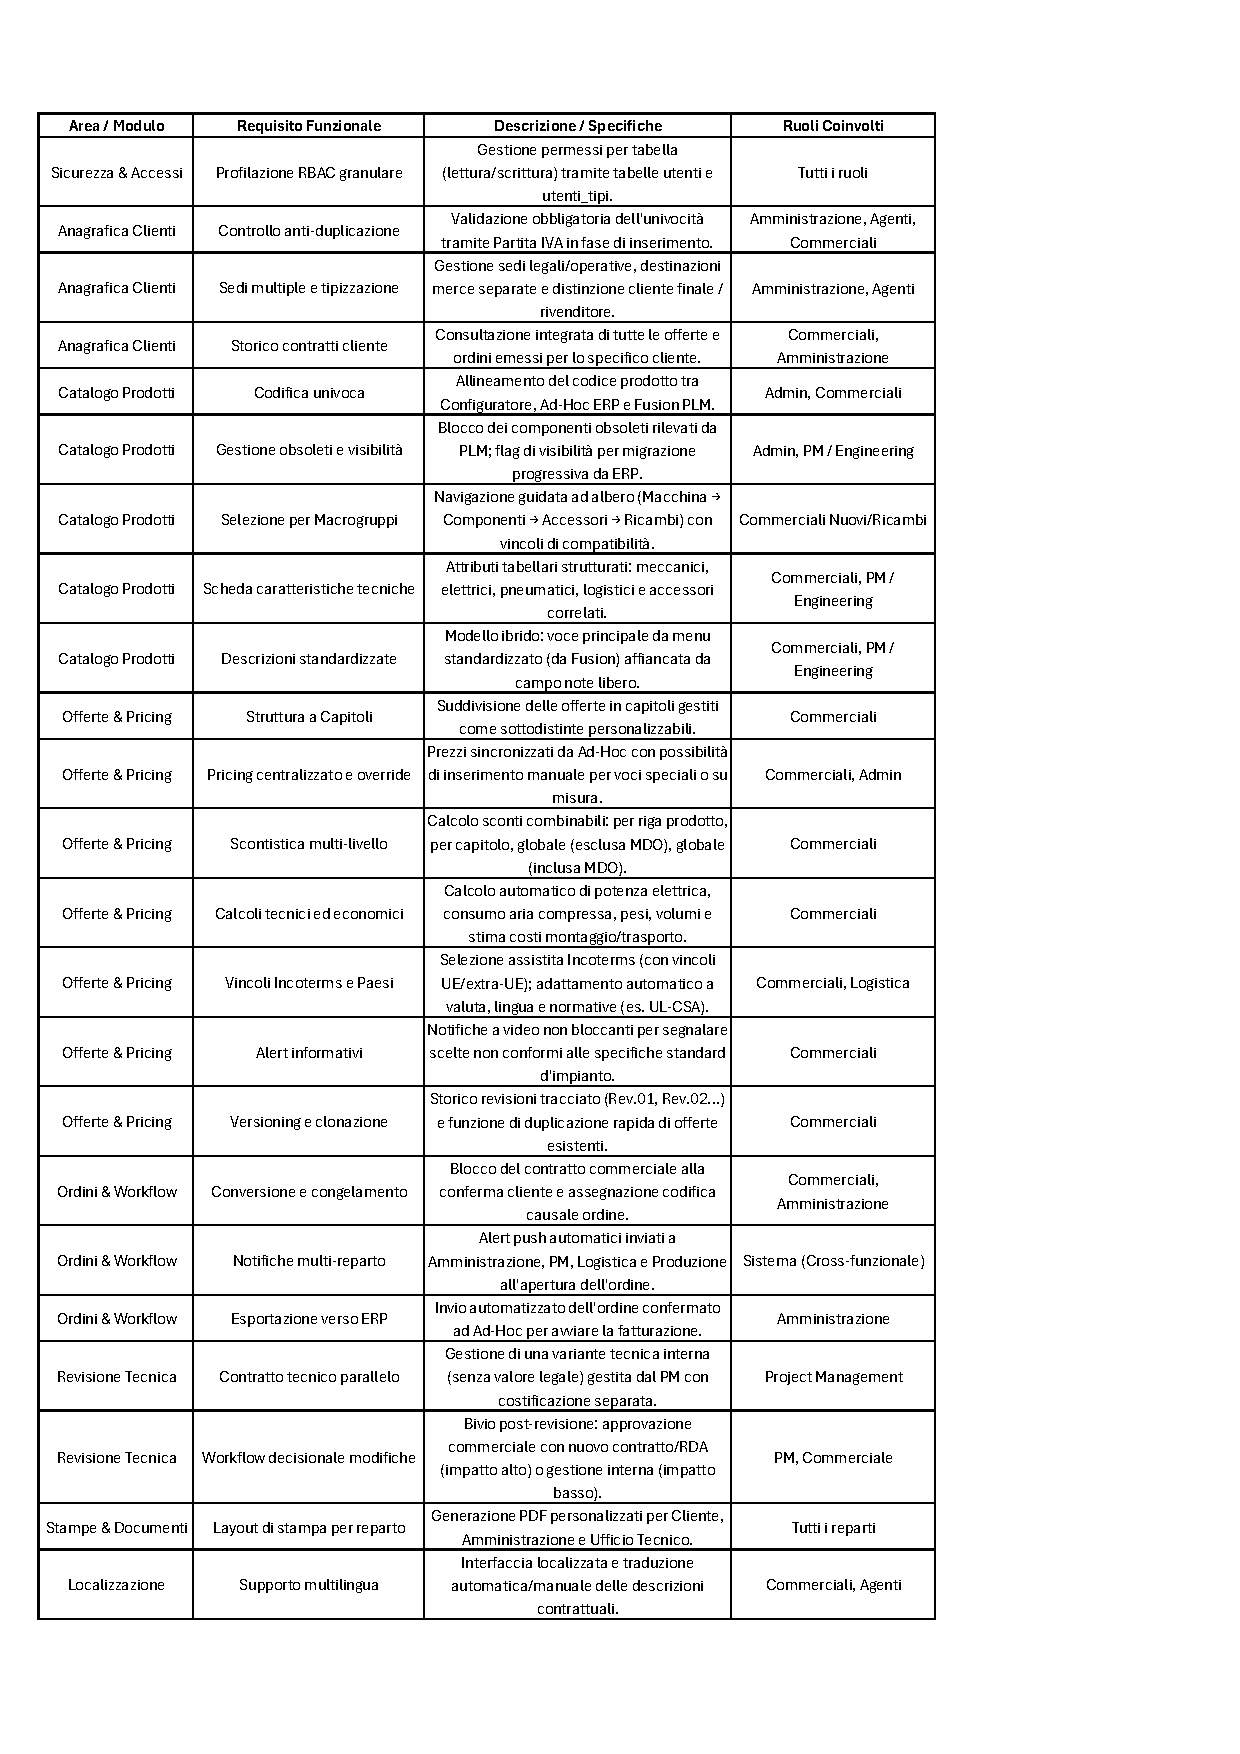
\includegraphics[width=0.9\linewidth]{Tabelle/RequisitiFunzionali.pdf}
    \caption{Requisiti funzionali raccolti.}
    \label{fig:Requisiti funzionali}
\end{figure}
\section{Requisiti non funzionali}

\begin{figure}[h]
    \centering
    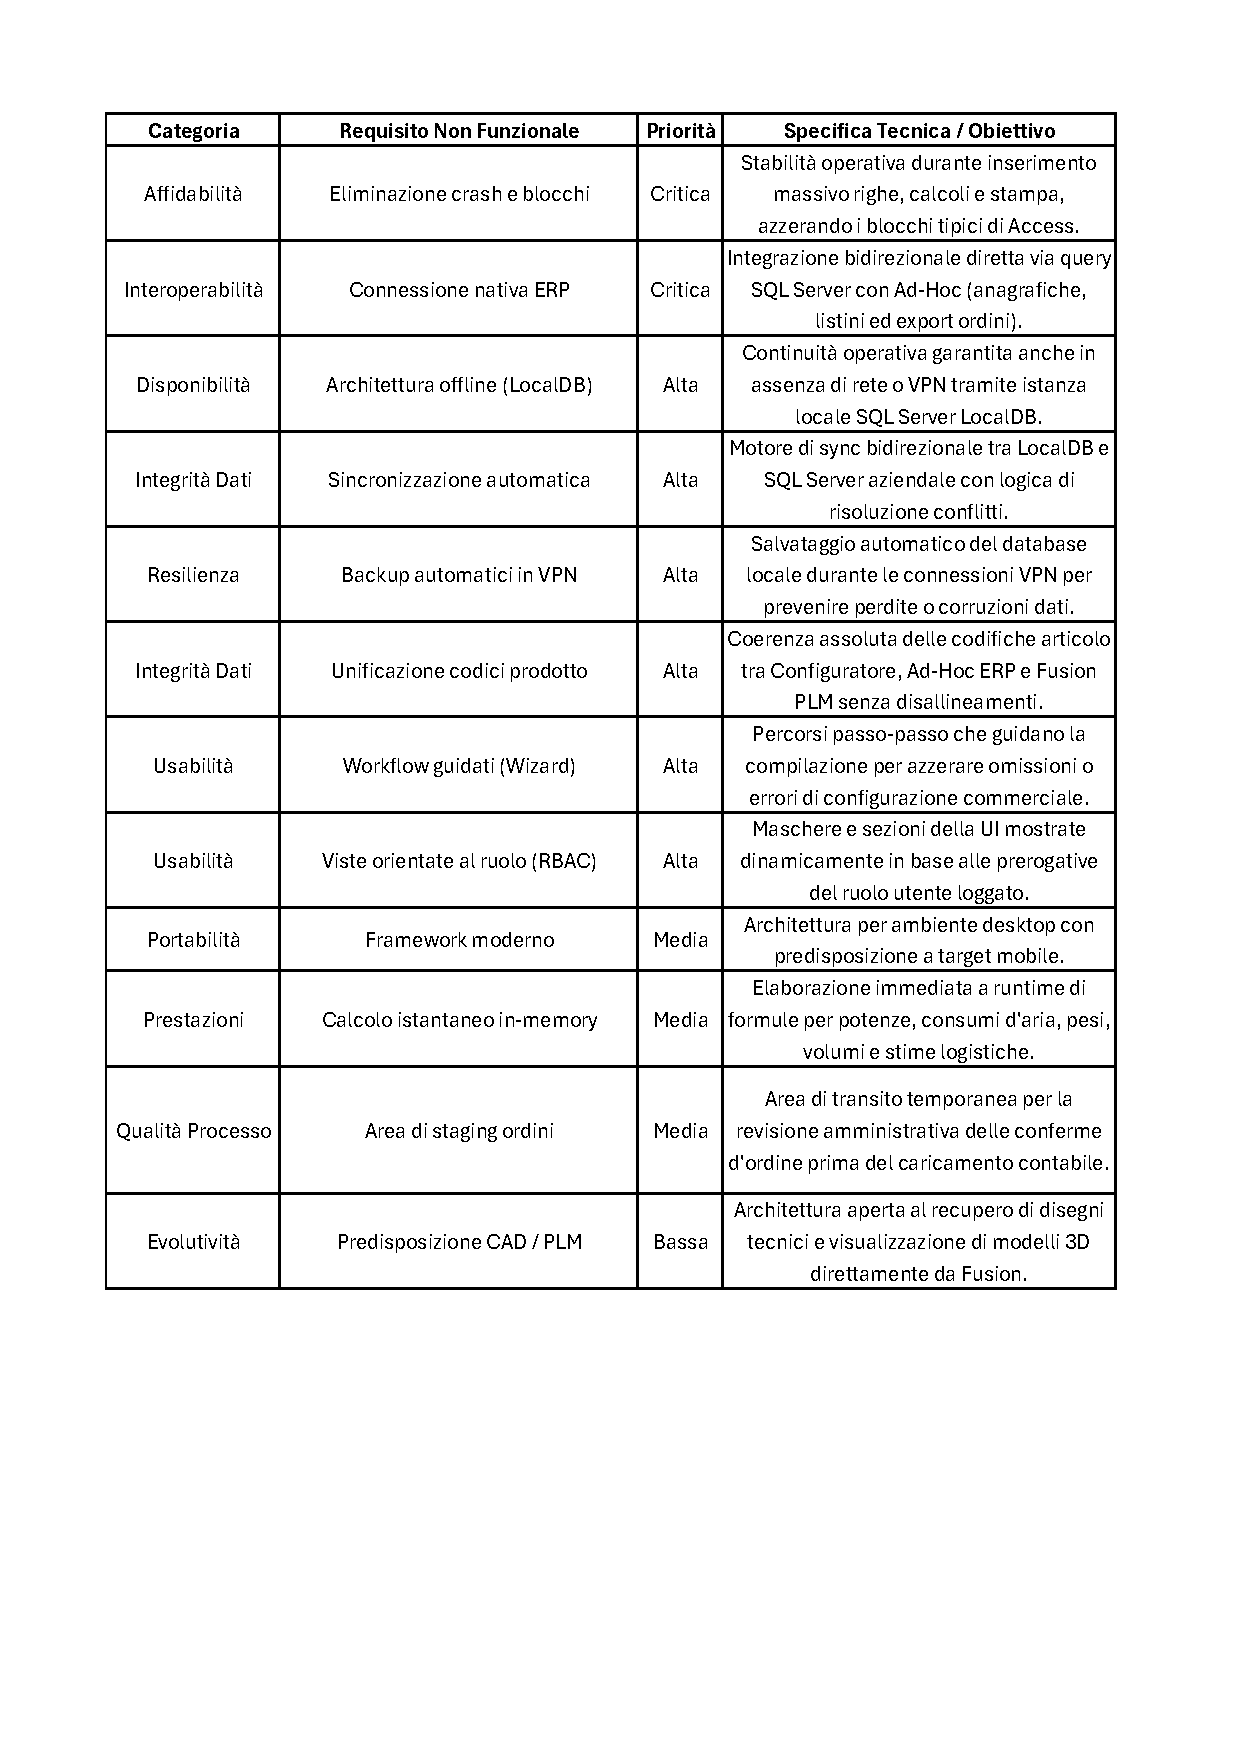
\includegraphics[width=0.9\linewidth]{Tabelle/RequisitiNonFunzionali.pdf}
    \caption{Requisiti non funzionali raccolti.}
    \label{fig:Requisiti non funzionali}
\end{figure}
\section{Requisiti futuri should-have}